% -*- coding: utf-8 -*-
% !TEX program = xelatex
\documentclass[10pt,a4paper]{article}
\usepackage{geometry}
\geometry{left=2.5cm,right=2.5cm,top=2.5cm,bottom=2.5cm}

\usepackage{multicol}
%\usepackage{fontspec}
\usepackage[most]{tcolorbox}
\newcounter{testexample}
\usepackage{xparse}
\usepackage{lipsum}
\usepackage[UTF8,noindent]{ctex}
\usepackage{extarrows}
%\usepackage{courier}
\usepackage{animate}
\usepackage{dcolumn}
\usepackage{pgf}
\usepackage{tikz}
\usetikzlibrary{calc}
\usetikzlibrary{arrows,snakes,backgrounds,shapes,patterns}
\usetikzlibrary{matrix,fit,positioning,decorations.pathmorphing}
\usepackage{listings}
\lstset{
        language=python,
        keywordstyle=\color{blue!70},
        frame=single,
        basicstyle=\ttfamily,
        commentstyle=\color{red},
        breakindent=0pt,
        rulesepcolor=\color{red!20!green!20!blue!20},
        rulecolor=\color{black},
        tabsize=4,
        numbersep=5pt,
        breaklines=true,
        %% backgroundcolor=\color{red!10},
        showstringspaces=false,
        showspaces=false,
        showtabs=false,
        extendedchars=false,
        escapeinside=``,
        frame=single,
}
\def\exampletext{例} % If English
\NewDocumentEnvironment{testexample}{ O{} }
{
\colorlet{colexam}{red!55!black} % Global example color
\newtcolorbox[use counter=testexample]{testexamplebox}{%
    % Example Frame Start
    empty,% Empty previously set parameters
    title={\exampletext: #1},% use \thetcbcounter to access the testexample counter text
    % Attaching a box requires an overlay
    attach boxed title to top left,
       % Ensures proper line breaking in longer titles
       minipage boxed title,
    % (boxed title style requires an overlay)
    boxed title style={empty,size=minimal,toprule=0pt,top=4pt,left=3mm,overlay={}},
    coltitle=colexam,fonttitle=\bfseries,
    before=\par\medskip\noindent,parbox=false,boxsep=0pt,left=3mm,right=0mm,top=2pt,breakable,pad at break=0mm,
       before upper=\csname @totalleftmargin\endcsname0pt, % Use instead of parbox=true. This ensures parskip is inherited by box.
    % Handles box when it exists on one page only
    overlay unbroken={\draw[colexam,line width=.5pt] ([xshift=-0pt]title.north west) -- ([xshift=-0pt]frame.south west); },
    % Handles multipage box: first page
    overlay first={\draw[colexam,line width=.5pt] ([xshift=-0pt]title.north west) -- ([xshift=-0pt]frame.south west); },
    % Handles multipage box: middle page
    overlay middle={\draw[colexam,line width=.5pt] ([xshift=-0pt]frame.north west) -- ([xshift=-0pt]frame.south west); },
    % Handles multipage box: last page
    overlay last={\draw[colexam,line width=.5pt] ([xshift=-0pt]frame.north west) -- ([xshift=-0pt]frame.south west); },%
    }
\begin{testexamplebox}}
{\end{testexamplebox}\endlist}




\begin{document}

\title{介绍}
% \author{张晓平}
% \date{}                                           % Activate to display a given date or no date
\maketitle

\section{目标}
\begin{itemize}
\item 回顾计算机科学的思想, 提高编程和解决问题的能力。
\item 理解抽象化以及它在解决问题过程中发挥的作用
\item 理解和实现抽象数据类型的概念
\item 回顾 Python 编程语言
\end{itemize}

\section{快速开始}

从第一台通过接入网线和交换机来传递人的指令的计算机开始,我们编程思考的方式发生了许多变化。与社会的许多方面一样,计算技术的变化为计算机科学家提供了越来越多的工具和平台来实践他们的工艺。计算机的快速发展诸如更快的处理器,高速网络和大的存储器容量已经让计算机科学家陷入高度复杂螺旋中。在所有这些快速演变中,一些基本原则保持不变。计算机科学关注用计算机来解决问题。
毫无疑问你花了相当多的时间学习解决问题的基础知识,以此希望有足够的能力把问题弄清楚并想出解决方案。你还发现编写代码通常很困难。问题的复杂性和解决方案的相应复杂性往往会掩盖与解决问题过程相关的基本思想。
本章着重介绍了其他两个重要的部分。首先回顾了计算机科学与算法和研究数据结构所必须适应的框架,特别是我们需要研究这些主题的原因,以及如何理解这些主题有助于我们更好的解决问题。第二,我们回顾 Python 编程语言。虽然我们不提供详尽的参考,我们将在其余章节中给出基本数据结构的示例和解释。 


\section{什么是计算机科学}

计算机科学往往难以定义。这可能是由于在名称中不幸使用了“计算机”一词。正如你可能知道的,计算机科学不仅仅是计算机的研究。虽然计算机作为一个工具在学科中发挥重要的支持作用,但它们只是工具。
计算机科学是对问题,解决问题以及解决问题过程中产生的解决方案的研究。给定一个问题,计算机科学家的目标是开发一个算法,一系列的指令列表,用于解决可能出现的问题的任何实例。算法遵循它有限的过程就可以解决问题。
计算机科学可以被认为是对算法的研究。但是,我们必须谨慎地包括一些事实,即一些问题可能没有解决方案。虽然证明这种说法正确性超出了本文的范围,但一些问题不能解决的事实对于那些研究计算机科学的人是很重要的。所以我们可以这么定义计算机科学,是研究能被解决的问题的方案和不能被解决问题的科学。
通常我们会说这个问题是可计算的,当在描述问题和解决方案时。如果存在一个算法解决这个问题,那么问题是可计算的。计算机科学的另一个定义是说,计算机科学是研究那些可计算和不可计算的问题,研究是不是存在一种算法来解决它。你会注意到,“电脑”一词根本没有出现。解决方案是独立于机器而言的。
计算机科学,因为它涉及问题解决过程本身,也是抽象的研究。抽象使我们能够以分离所谓的逻辑和物理角度的方式来观察问题和解决方案。基本思想跟我们常见的例子一样。
假设你可能已经开车上学或上班。作为司机,汽车的用户。你为了让汽车载你到目的地,你会和汽车有些互动。进入汽车,插入钥匙,点火,换挡,制动,加速和转向。从抽象的角度,我们可以说你所看到的是汽车的逻辑视角。你正在使用汽车设计师提供的功能,将你从一个地方运输到另一个位置。这些功能有时也被称为接口。
另一方面,修理汽车的技工有一个截然不同的视角。他不仅知道如何开车,还必须知道所有必要的细节,使我们认为理所当然的功能运行起来。他需要了解发动机是如何工作的,变速箱如何变速,温度是如何控制的等等。这被称为物理视角,细节发生在“引擎盖下”。
当我们使用电脑时也会发生同样的情况。大多数人使用计算机写文档,发送和接收电子邮件,上网冲浪,播放音乐,存储图像和玩游戏,而不知道让这些应用程序工作的细节。他们从逻辑或用户角度看计算机。计算机科学家,程序员,技术支持人员和系统管理员看计算机的角度截然不同。他们必须知道操作系统如何工作的细节,如何配置网络协议,以及如何编写控制功能的各种脚本。他们必须能够控制底层的细节。
这两个示例的共同点是用户态的抽象,有时也称为客户端,不需要知道细节,只要用户知道接口的工作方式。这个接口是用户与底层沟通的方式。作为抽象的另一个例子,Python 数学模块。一旦我们导入模块,我们可以执行计算
\begin{lstlisting}
>>> import math
>>> math.sqrt(16)
4.0
>>>
\end{lstlisting}

这是一个程序抽象的例子。我们不一定知道如何计算平方根,但我们知道函数是什么以及如何使用它。如果我们正确地执行导入,我们可以假设该函数将为我们提供正确的结果。我们知道有人实现了平方根问题的解决方案,但我们只需要知道如何使用它。这有时被称为“黑盒子”视图。我们简单地描述下接口:函数的名称,需要什么(参数),以及将返回什么。细节隐藏在里面
\begin{figure}[htbp]
\centering
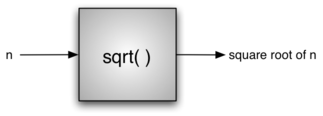
\includegraphics[width=3in]{images/blackbox.png}
\end{figure}


\section{什么是编程}
        
编程是将算法编码为符号,编程语言的过程,以使得其可以由计算机执行。虽然有许多编程语言和不同类型的计算机存在,第一步是需要有解决方案。没有算法就没有程序。

计算机科学不是研究编程。然而,编程是计算机科学家的一个重要能力。编程通常是我们为解决方案创建的表现形式。因此,这种语言表现形式和创造它的过程成为该学科的基本部分。
        
算法描述了依据问题实例数据所产生的解决方案和产生预期结果所需的一套步骤。编程语言必须提供一种表示方法来表示过程和数据。为此,它提供了控制结构和数据类型。
        
控制结构允许以方便而明确的方式表示算法步骤。至少,算法需要执行顺序处理,决策选择和重复控制迭代。只要语言提供这些基本语句,它就可以用于算法表示。
        
计算机中的所有数据项都以二进制形式表示。为了赋给这些字符串含义,我们需要有数据类型。数据类型提供了对这个二进制数据的解释,以便我们能够根据解决的问题思考数据。这些底层的内置数据类型(有时称为原始数据类型)为算法开发提供了基础。
        
例如,大多数编程语言为整数提供数据类型。内存中的二进制数据可以解释为整数,并且能给予一个我们通常与整数(例如 23,654 和 -19)相关联的含义。此外,数据类型还提供数据项参与的操作的描述。对于整数,诸如加法,减法和乘法的操作是常见的。我们期望数值类型的数据可以参与这些算术运算。通常我们遇到的困难是问题及其解决方案非常复杂。这些简单的,语言提供的结构和数据类型虽然足以表示复杂的解决方案,但通常在我们处理问题的过程中处于不利地位。我们需要一些方法控制这种复杂性,并能给我们提供更好的解决方案。
        
\section{为什么要学习数据结构和抽象数据类型}

为了管理问题的复杂性和解决问题的过程,计算机科学家使用抽象使他们能够专注于 “大局” 而不会迷失在细节中。通过创建问题域的模型,我们能够利用更好和更有效的问题解决过程。这些模型允许我们以更加一致的方式描述我们的算法将要处理的数据。
之前,我们将过程抽象称为隐藏特定函数的细节的过程,以允许用户或客户端在高层查看它。我们现在将注意力转向类似的思想,即数据抽象的思想。抽象数据类型(有时缩写为 ADT )是对我们如何查看数据和允许的操作的逻辑描述,而不用考虑如何实现它们。这意味着我们只关心数据表示什么,而不关心它最终将如何构造。通过提供这种级别的抽象,我们围绕数据创建一个封装。通过封装实现细节,我们将它们从用户的视图中隐藏。这称为信息隐藏。
\begin{figure}[htbp]
        \centering
        
\includegraphics[width=6in]{images/ds_adt.png}
\end{figure}

Figure 2 展示了抽象数据类型是什么以及如何操作。用户与接口交互,使用抽象数据类型指定的操作。抽象数据类型是用户与之交互的 shell。实现隐藏在更深的底层。用户不关心实现的细节。 



抽象数据类型(通常称为数据结构)的实现将要求我们使用一些程序构建和原始数据类型的集合来提供数据的物理视图。 正如我们前面讨论的,这两个视角的分离将允许我们将问题定义复杂的数据模型,而不给出关于模型如何实际构建的细节。 这提供了独立于实现的数据视图。由于通常有许多不同的方法来实现抽象数据类型,所以这种实现独立性允许程序员在不改变数据的用户与其交互的方式的情况下切换实现的细节。 用户可以继续专注于解决问题的过程。


\section{为什么要学习算法}

计算机科学家经常通过经验学习。我们通过看别人解决问题和自己解决问题来学习。接触不同的问题解决技术,看不同的算法设计有助于我们承担下一个具有挑战性的问题。通过思考许多不同的算法,我们可以开始开发模式识别,以便下一次出现类似的问题时,我们能够更好地解决它。
算法通常彼此完全不同。考虑前面看到的 sqrt 的例子。完全可能的是,存在许多不同的方式来实现细节以计算平方根函数。一种算法可以使用比另一种更少的资源。一个算法可能需要 10 倍的时间来返回结果。我们想要一些方法来比较这两个解决方案。即使他们都工作,一个可能比另一个“更好”。我们建议使用一个更高效,或者一个只是工作更快或使用更少的内存的算法。当我们研究算法时,我们可以学习分析技术,允许我们仅仅根据自己的特征而不是用于实现它们的程序或计算机的特征来比较和对比解决方案。
在最坏的情况下,我们可能有一个难以处理的问题,这意味着没有算法可以在实际的时间量内解决问题。重要的是能够区分具有解决方案的那些问题,不具有解决方案的那些问题,以及存在解决方案但需要太多时间或其他资源来合理工作的那些问题。
经常需要权衡,我们需要做决定。作为计算机科学家,除了我们解决问题的能力,我们还需要了解解决方案评估技术。最后,通常有很多方法来解决问题。找到一个解决方案,我们将一遍又一遍比较,然后决定它是否是一个好的方案。


\section{Python介绍}

%Python is a high-level, dynamically typed multiparadigm programming language. Python code is often said to be almost like pseudocode, since it allows you to express very powerful ideas in very few lines of code while being very readable. As an example, here is an implementation of the classic quicksort algorithm in Python:

Python 是一种高级的、动态的多范型编程语言。Python代码很多时候看起来就像是伪代码一样,因此你可以使用很少的几行可读性很高的代码来实现一个非常强大的想法。举个例子,下面是使用Python来实现非常经典的快速排序算法的代码。

\lstinputlisting[]{code/quicksort.py}

\subsection{Python versions}

%There are currently two different supported versions of Python, 2.7 and 3.5. Somewhat confusingly, Python 3.0 introduced many backwards-incompatible changes to the language, so code written for 2.7 may not work under 3.5 and vice versa. For this class all code will use Python 3.5.
%
%You can check your Python version at the command line by running 


目前有两种不同的Python版本被支持,分别是2.7和3.4。令人不解的是,Python 3.0引入了一些不可向下兼容的变换,所以使用2.7写的代码不一定能在3.4版本上运行,反之亦然。%在本课程中代码都是运行在2.7版本上的。

你可以在命令行中使用一下命令来检查一下自己的Python版本:

\begin{lstlisting}
python --version
\end{lstlisting}



\subsection{基本数据类型}

%Like most languages, Python has a number of basic types including integers, floats, booleans, and strings. These data types behave in ways that are familiar from other programming languages.
%
%Numbers: Integers and floats work as you would expect from other languages:
%

和很多语言一样,Python 也有几种数据类型包括:整型、浮点型、布尔型和字符型。这些数据类型的表现方式和大家熟悉的其他语言一样。


\subsubsection{Numbers}
整型和浮点型的工作方式和其他语言一样。

\lstinputlisting[]{code/numbers.py}

%Note that unlike many languages, Python does not have unary increment (x++) or decrement (x--) operators.
%
%Python also has built-in types for complex numbers; you can find all of the details in the documentation.

注意:Python没有类似于\lstinline|++|和\lstinline|--|的一元运算的操作。 Python也内置了长整型和复数。


%Booleans: Python implements all of the usual operators for Boolean logic, but uses English words rather than symbols (\lstinline|&&, |||, etc.):
%

\subsubsection{Booleans}
Python的布尔型逻辑和其他语言都一样,不过使用了英文单词替换了符号(\lstinline|&&, |||, etc.):


\lstinputlisting[]{code/boolean.py}
%
%Strings: Python has great support for strings:

\subsubsection{Strings}
Python 对字符型的支持非常强大。

\lstinputlisting[]{code/string1.py}

%String objects have a bunch of useful methods; for example:

String 对象还有很多常用的方法,例如:

\lstinputlisting[]{code/string2.py}


\subsection{容器(Containers)}

%Python includes several built-in container types: lists, dictionaries, sets, and tuples.
Python包含了几个内置的容器类型:列表(lists)、字典(dictionaries)、集合(sets)、 元组(tuples)

\subsubsection{列表(list)}

%A list is the Python equivalent of an array, but is resizeable and can contain elements of different types:

list在Python中几乎等价于数组,但是是可调整大小的同时也可以包容不同类型的元素。


\lstinputlisting[]{code/list.py}

%Slicing: In addition to accessing list elements one at a time, Python provides concise syntax to access sublists; this is known as slicing:

切片(Slicing):除了每次访问一个列表元素,Python还提供了一种简洁的语法去访问子列表,这被称为slicing:


\lstinputlisting[]{code/list_slices.py}

%We will see slicing again in the context of numpy arrays.

我们将会在numpy arrays章节中再看到slicing.


%Loops: You can loop over the elements of a list like this:

Loops:你可以用如下方法遍历列表元素:

\lstinputlisting[]{code/list_loops.py}

%If you want access to the index of each element within the body of a loop, use the built-in enumerate function:

如果你想使用循环结构得到元素的索引以及内容,使用内置的“enumerate”方法

\lstinputlisting[]{code/list_enumerate.py}


%List comprehensions: When programming, frequently we want to transform one type of data into another. As a simple example, consider the following code that computes square numbers:

列表推导:在编程的时候我们经常会想要将一种数据类型转换成另一种。举个简单的例子,思考下面这段代码,它计算了数据的平方:


\lstinputlisting[]{code/list_comprehensions.py}

%You can make this code simpler using a list comprehension:

你也可以使用列表推导写出更简单的代码:

\lstinputlisting[]{code/list_comprehensions1.py}

%List comprehensions can also contain conditions:

列表推导还可以包含判断逻辑:

\lstinputlisting[]{code/list_comprehensions2.py}


\subsubsection{字典(Dictionaries)}

%A dictionary stores (key, value) pairs, similar to a Map in Java or an object in Javascript. You can use it like this:

字典由键值对组成。就像JAVA里面的map,以及JavaScript中的Object。使用方法如下:

\lstinputlisting[]{code/dict.py}


%Loops: It is easy to iterate over the keys in a dictionary:

Loops:根据字典的键很容易进行迭代。
\lstinputlisting[]{code/dict_loops.py}

%If you want access to keys and their corresponding values, use the items method:

如果你想获得键以及对应的值,使用items方法
\lstinputlisting[]{code/dict_items.py}

%Dictionary comprehensions: These are similar to list comprehensions, but allow you to easily construct dictionaries. For example:

字典推导(Dictionary comprehensions): 和推导列表差不多,不过可以更简单的构建字典。

\lstinputlisting[]{code/dict_comprehensions.py}

\subsubsection{集合(Sets)}

%A set is an unordered collection of distinct elements. As a simple example, consider the following:

sets是离散元的无序集合。下面举个简单的例子

\lstinputlisting[]{code/set.py}

%Loops: Iterating over a set has the same syntax as iterating over a list; however since sets are unordered, you cannot make assumptions about the order in which you visit the elements of the set:

Loops:迭代集合的语法和迭代列表的一样,但是当集合是无序的时候,在便利集合中的元素时不要有排序的预期。
\lstinputlisting[]{code/set_loops.py}

%Set comprehensions: Like lists and dictionaries, we can easily construct sets using set comprehensions:

集合推导(Set comprehensions): 和列表以及字典一样。我们可以很简单的构建一个集合:
\lstinputlisting[]{code/set_comprehensions.py}

\subsubsection{元组(Tuples)}

%A tuple is an (immutable) ordered list of values. A tuple is in many ways similar to a list; one of the most important differences is that tuples can be used as keys in dictionaries and as elements of sets, while lists cannot. Here is a trivial example:

元组是一个有序列表。在很多方面和列表一样,有一点非常重要的不同就是元组可以在字典中被用作键而列表不行。例子:
\lstinputlisting[]{code/tuple.py}


\subsubsection{函数}

%Python functions are defined using the def keyword. For example:

python 中函数的定义使用 def 关键字,如:
\lstinputlisting[]{code/def.py}

%We will often define functions to take optional keyword arguments, like this:

我们将会用到带有可选参数的方法,例如:
\lstinputlisting[]{code/hello.py}


\subsubsection{类}

%The syntax for defining classes in Python is straightforward:

定义类的语法在Python中很简单:


\lstinputlisting[]{code/class.py}


\section{Numpy}

%Numpy is the core library for scientific computing in Python. It provides a high-performance multidimensional array object, and tools for working with these arrays. If you are already familiar with MATLAB, you might find this tutorial useful to get started with Numpy.

Numpy 是 Python 中科学计算的核心库。它提供一个高性能多维数据对象,以及操作这个对象的工具。如果你已经熟悉了 MATLAB ,你会发现本教程对于 numpy 起步很有用。

\subsection{数组}

%A numpy array is a grid of values, all of the same type, and is indexed by a tuple of nonnegative integers. The number of dimensions is the rank of the array; the shape of an array is a tuple of integers giving the size of the array along each dimension.
%
%We can initialize numpy arrays from nested Python lists, and access elements using square brackets:

Numpy数组可以理解为一个矩阵,所有元素的类型都是一样的,是一个被索引的非负整数的元组。数组的维度大小是数组的 rank ,数组的 shape 是一个整型的元组,给出每个维度数组的大小。

我们可以使用嵌套 Python 列表来初始化一个 numpy 数组,使用方括号来访问元素。


\lstinputlisting[]{code/np_array1.py}

%Numpy also provides many functions to create arrays:

Numpy还提供很多方法来创建数组:
\lstinputlisting[]{code/np_array2.py}


\subsection{数组索引}

%Numpy offers several ways to index into arrays.
%
%Slicing: Similar to Python lists, numpy arrays can be sliced. Since arrays may be multidimensional, you must specify a slice for each dimension of the array:

Numpy提供了多种方法来索引数组。

切片:和Python的列表一样numpy数组也是可以被切片的。因为数组可能是多维的,所以对数组的每一个元素都要指定切片:


\lstinputlisting[]{code/np_array_slice.py}


%You can also mix integer indexing with slice indexing. However, doing so will yield an array of lower rank than the original array. Note that this is quite different from the way that MATLAB handles array slicing:

你也可以混合整型索引和切片索引。然而这样做将会得到一个相比原始数组rank更低的数组。注意这和MATLAB处理数组切片的方法有很大的不同。

\lstinputlisting[]{code/np_array_shape.py}



%Integer array indexing: When you index into numpy arrays using slicing, the resulting array view will always be a subarray of the original array. In contrast, integer array indexing allows you to construct arbitrary arrays using the data from another array. Here is an example:

整型数组索引:当你使用切片来索引numpy数组时,结果的数组视图总是源数组的子数组。相比之下,整型数组索引允许您使用其他数组的数据构建任意数组。例如:


\lstinputlisting[]{code/np_integer_array_index.py}

%One useful trick with integer array indexing is selecting or mutating one element from each row of a matrix:

整型数组索引的一个实用技巧是用来选择或变换矩阵的每一行的一个元素。
\lstinputlisting[]{code/np_integer_array_index1.py}


%Boolean array indexing: Boolean array indexing lets you pick out arbitrary elements of an array. Frequently this type of indexing is used to select the elements of an array that satisfy some condition. Here is an example:

布尔数组索引:布尔数组索引可以取得一个数组中的任意元素。通常这种索引方式用来选择符合一定条件的元素。例如:

\lstinputlisting[]{code/np_boolean_array_index.py}


\subsection{数据类型}

Every numpy array is a grid of elements of the same type. Numpy provides a large set of numeric datatypes that you can use to construct arrays. Numpy tries to guess a datatype when you create an array, but functions that construct arrays usually also include an optional argument to explicitly specify the datatype. Here is an example:
\lstinputlisting[]{code/np_datatype.py}

\subsection{Array math}

Basic mathematical functions operate elementwise on arrays, and are available both as operator overloads and as functions in the numpy module:



\lstinputlisting[]{code/np_array_math.py}


%Note that unlike MATLAB, * is elementwise multiplication, not matrix multiplication. We instead use the dot function to compute inner products of vectors, to multiply a vector by a matrix, and to multiply matrices. dot is available both as a function in the numpy module and as an instance method of array objects:

注意:不同于MATLAB,* 是逐点乘法,而不是矩阵乘法。我们使用 dot 函数计算向量的的内积、将一个向量乘以一个矩阵、矩阵乘以矩阵。dot 可作为 numpy 模块的一个函数,也可以作为数组对象的一个实例方法:
\lstinputlisting[]{code/np_dot.py}

%Numpy provides many useful functions for performing computations on arrays; one of the most useful is sum:

Numpy 提供很多有用的函数来实现数组的运算;其中一个最有用的就是 sum :
\lstinputlisting[]{code/np_sum.py}


%Apart from computing mathematical functions using arrays, we frequently need to reshape or otherwise manipulate data in arrays. The simplest example of this type of operation is transposing a matrix; to transpose a matrix, simply use the T attribute of an array object:

除了利用数组计算数学函数,我们还经常需要对数组进行reshape或处理其中的数据。关于这类操作最简单的例子就是矩阵的转置;去转置一个矩阵,只需使用数组对象的T属性:
\lstinputlisting[]{code/np_transpose.py}


\subsection{广播机制(Broadcasting)}


Broadcasting is a powerful mechanism that allows numpy to work with arrays of different shapes when performing arithmetic operations. Frequently we have a smaller array and a larger array, and we want to use the smaller array multiple times to perform some operation on the larger array.

For example, suppose that we want to add a constant vector to each row of a matrix. We could do it like this:

广播是一种强大的机制,它允许numpy在实现算术操作时去处理不同不同shape的数组。假设有一个小数组和一个大数组,我们想多次使用小数组去对大数组做某些操作。例如,假设我们想对矩阵的每一行加上一个常向量,可以这么做:
\lstinputlisting[]{code/np_broadcast.py}


%This works; however when the matrix x is very large, computing an explicit loop in Python could be slow. Note that adding the vector v to each row of the matrix x is equivalent to forming a matrix vv by stacking multiple copies of v vertically, then performing elementwise summation of x and vv. We could implement this approach like this:

可以这么做;然而当矩阵 x 很大时,在 Python 中计算一个显示的循环会很慢。注意对矩阵 x 的每一行加上向量 v 等价于通过按垂直方向复制 v 若干次而叠加成一个矩阵 vv,然后对 x 和 vv 进行逐元加法。我们可以这样实现这一过程: 


\lstinputlisting[]{code/np_broadcast1.py}


%Numpy broadcasting allows us to perform this computation without actually creating multiple copies of v. Consider this version, using broadcasting:

Numpy 广播机制允许我们不需要真正地创建v的多重拷贝来执行这一计算。使用广播机制,我们可以这么做:

\lstinputlisting[]{code/np_broadcast2.py}


%The line y = x + v works even though x has shape (4, 3) and v has shape (3,) due to broadcasting; this line works as if v actually had shape (4, 3), where each row was a copy of v, and the sum was performed elementwise.

由于广播机制,即使 x 有shape (4, 3), v 有shape (3,),行\lstinline|y = x + v| 仍可工作; 这就如同 v 有shape (4, 3),其中每一行为v的拷贝,求和按逐元进行。



Broadcasting two arrays together follows these rules:
\begin{enumerate}
\item If the arrays do not have the same rank, prepend the shape of the lower rank array with 1s until both shapes have the same length.
\item The two arrays are said to be compatible in a dimension if they have the same size in the dimension, or if one of the arrays has size 1 in that dimension.
\item The arrays can be broadcast together if they are compatible in all dimensions.
\item After broadcasting, each array behaves as if it had shape equal to the elementwise maximum of shapes of the two input arrays.
\item In any dimension where one array had size 1 and the other array had size greater than 1, the first array behaves as if it were copied along that dimension
\item If this explanation does not make sense, try reading the explanation from the documentation or this explanation.
\end{enumerate}

广播两个数组遵循以下原则:
\begin{enumerate}
        \item If the arrays do not have the same rank, prepend the shape of the lower rank array with 1s until both shapes have the same length.
        当两个数组的rank不一致时,
        \item The two arrays are said to be compatible in a dimension if they have the same size in the dimension, or if one of the arrays has size 1 in that dimension.
        \item The arrays can be broadcast together if they are compatible in all dimensions.
        \item After broadcasting, each array behaves as if it had shape equal to the elementwise maximum of shapes of the two input arrays.
        \item In any dimension where one array had size 1 and the other array had size greater than 1, the first array behaves as if it were copied along that dimension
        \item If this explanation does not make sense, try reading the explanation from the documentation or this explanation.
\end{enumerate}


Functions that support broadcasting are known as universal functions. You can find the list of all universal functions in the documentation.

Here are some applications of broadcasting:
\lstinputlisting[]{code/np_broadcast3.py}

Broadcasting typically makes your code more concise and faster, so you should strive to use it where possible.


\section{SciPy}

Numpy provides a high-performance multidimensional array and basic tools to compute with and manipulate these arrays. SciPy builds on this, and provides a large number of functions that operate on numpy arrays and are useful for different types of scientific and engineering applications.

The best way to get familiar with SciPy is to browse the documentation. We will highlight some parts of SciPy that you might find useful for this class.


\subsection{Image operations}

SciPy provides some basic functions to work with images. For example, it has functions to read images from disk into numpy arrays, to write numpy arrays to disk as images, and to resize images. Here is a simple example that showcases these functions:
\lstinputlisting[]{code/scipy_misc.py}

\begin{figure}[htbp]
\centering

\includegraphics[width=2in]{images/cat.jpg}

\includegraphics[width=2in]{images/cat_tinted.jpg}
\end{figure}

\subsection{MATLAB files}

The functions scipy.io.loadmat and scipy.io.savemat allow you to read and write MATLAB files. You can read about them in the documentation.


\subsection{Distance between points}

SciPy defines some useful functions for computing distances between sets of points.


The function scipy.spatial.distance.pdist computes the distance between all pairs of points in a given set:


A similar function (scipy.spatial.distance.cdist) computes the distance between all pairs across two sets of points; you can read about it in the documentation.
\lstinputlisting[]{code/scipy_pdist.py}

\section{Matplotlib}

Matplotlib is a plotting library. In this section give a brief introduction to the matplotlib.pyplot module, which provides a plotting system similar to that of MATLAB.


\subsection{Plotting}

The most important function in matplotlib is plot, which allows you to plot 2D data. Here is a simple example:
\lstinputlisting[]{code/matplotlib_plot.py}

Running this code produces the following plot:
\begin{figure}[htbp]
        \centering
        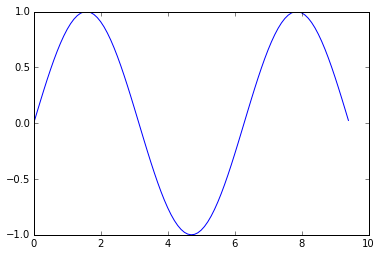
\includegraphics[width=2in]{images/sine.png}
\end{figure}



With just a little bit of extra work we can easily plot multiple lines at once, and add a title, legend, and axis labels:
\lstinputlisting[]{code/matplotlib_plot1.py}

\subsection{Subplots}

You can plot different things in the same figure using the subplot function. Here is an example:
\lstinputlisting[]{code/matplotlib_subplot.py}

\begin{figure}[htbp]
        \centering
        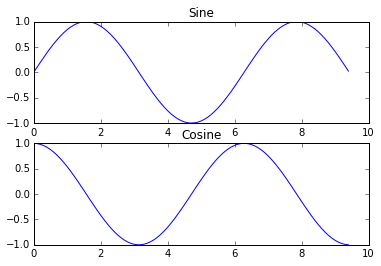
\includegraphics[width=2in]{images/sine_cosine_subplot.png}
\end{figure}


\subsection{Images}

You can use the imshow function to show images. Here is an example:
\lstinputlisting[]{code/matplotlib_imshow.py}

\begin{figure}[htbp]
        \centering
        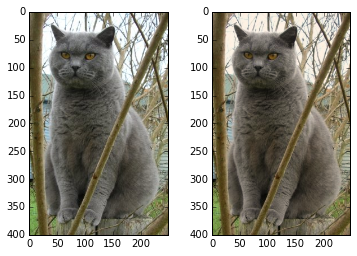
\includegraphics[width=4in]{images/cat_tinted_imshow.png}
\end{figure}

\end{document}